%%%%%%%%%%%%%%%%%%%%%%%%%%%%%%%%%%%%%%%%%
% fphw Assignment
% LaTeX Template
% Version 1.0 (27/04/2019)
%
% This template originates from:
% https://www.LaTeXTemplates.com
%
% Authors:
% Class by Felipe Portales-Oliva (f.portales.oliva@gmail.com) with template 
% content and modifications by Vel (vel@LaTeXTemplates.com)
%
% Template (this file) License:
% CC BY-NC-SA 3.0 (http://creativecommons.org/licenses/by-nc-sa/3.0/)
%
%%%%%%%%%%%%%%%%%%%%%%%%%%%%%%%%%%%%%%%%%

%----------------------------------------------------------------------------------------
%	PACKAGES AND OTHER DOCUMENT CONFIGURATIONS
%----------------------------------------------------------------------------------------

\documentclass[
	12pt, % Default font size, values between 10pt-12pt are allowed
	%letterpaper, % Uncomment for US letter paper size
	%spanish, % Uncomment for Spanish
]{fphw}

% Template-specific packages
\usepackage[utf8]{inputenc} % Required for inputting international characters
\usepackage[T1]{fontenc} % Output font encoding for international characters
\usepackage{mathpazo} % Use the Palatino font

\usepackage{graphicx} % Required for including images

\usepackage{booktabs} % Required for better horizontal rules in tables

\usepackage{listings} % Required for insertion of code

\usepackage{enumerate} % To modify the enumerate environment

\usepackage{leadsheets}

\usepackage{xcolor}

\usepackage{float}

\usepackage{caption}
\captionsetup[figure]{font=small}

%----------------------------------------------------------------------------------------
%	ASSIGNMENT INFORMATION
%----------------------------------------------------------------------------------------

\title{Homework \#2 - Template-Based Chord Recognition} % Assignment title

\author{Matteo Pettenò - Marco Viviani} % Students name

\date{December 23th, 2021} % Due date

\institute{Politecnico di Milano} % Institute or school name

\class{Computer Music - Representations and Models} % Course or class name

\professor{Clara Borrelli} % Professor or teacher in charge of the assignment

%----------------------------------------------------------------------------------------

\begin{document}

\maketitle % Output the assignment title, created automatically using the information in the custom commands above

%----------------------------------------------------------------------------------------
%	ASSIGNMENT CONTENT
%----------------------------------------------------------------------------------------

\color{red}
In generale: inglese da rivedere e check formattazione equazioni equazioni.
\color{black}

\section*{Introduzione}

In this report we analyze step by step the code implemented in the attached \emph{Jupyter Notebook} trying to answer the questions asked for this homework. Along with the reading of this report, please make sure to check out code comments in the notebook. The first cells of the notebook are used to initialize the context and the parameters of the algorithm.

\subsection*{Context initialization}
In order to optimize the code for automation and readability, in this section we initialize a dictionary that contains all the details of the songs used in the experiment (\emph{Corpus}). The chord labels are generated here too.

\subsection*{Parameters configuration}
In this cell we declare and set to a default value all the template-based chord recognition algorithm's parameters. This approach allows us to centralize the management of the algorithm's behavior, making it easier to evaluate once implemented.

\section*{\color{red}Question 1}

\begin{problem}
	\textbf{Implement the template based chord recognition algorithm.}
\end{problem}

\subsection*{\color{blue}Answer}

A chord recognition algorithm consists of two steps. In the first step, the given audio recording is cut into frames that are transformed into a feature vector. This is tipically done with chroma-based audio features, which contain the tonal information of the audio signal.
In the second step, pattern matching techniques are used to map each feature vector to a set of predefined chord models. The best fit determines the chord label assigned to the given frame.

\begin{figure}[H]
 \centering
 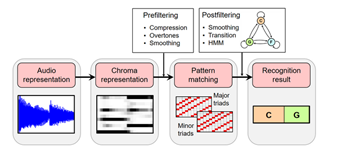
\includegraphics[scale=1]{./images/1_template_based_pipeline.png}
 \caption{Template-Based Chord Recognition Pipeline}
\end{figure}


\subsection*{Features processing functions}

\color{red}
Check punti 2, 3 e 4 che non siano troppo copiati.
\color{black}

In this section of the code all the functions that will be useful to implement features processing are defined. To improve the chord recognition results, in fact, additional enhancement techniques are applied either before the pattern matching step (\emph{prefiltering}) or after the pattern matching step (\emph{postfiltering}). In our implementation we only make use of prefiltering operations such as features compression, normalization, smoothing and downsampling.

\begin{enumerate}
	\item \verb|compress_feature_sequence| - This function takes in input the sequence of features and applies compression in a logarithmic fashion.
	\item \verb|normalize_feature_sequence| - This function normalizes the columns of a feature sequence. One normalization strategy is to choose a suitable norm  and then to replace each n-feature vector  by $x/p(x)$. The normalization procedure as described above replaces each chroma vector by its normalized version. Intuitively speaking, normalization introduces a kind of invariance to differences in dynamics or sound intensity. The normalization procedure is only possible if $p(x) \neq 0$. Also for very small values $p(x)$ which may occur in passages of silence before the actual start of the recording or during long pauses, normalization would lead to more or less random and therefore meaningless chroma value distributions. Therefore, if $p(x)$ calls below a certain threshold, the vector $x$ may be replaced by some standard vector such as a uniform vector of norm one instead of dividing by $p(x)$. In the function exactly this steps are implemented. Normalization will be used also in the post-processing phase in order to normalize the chord similarity matrix.
	\item \verb|smooth_feature_sequence| - For certain music retrieval applications, chromagrams may be too detailed. In particular, it may be desirable to further increase the similarity between them. This can be achieved by applying smoothing procedures. The idea is to compute for each chroma dimension a kind of local average over time. More precisely, let \(X=(x_1,x_2,...,x_N)\) be a feature sequence with $x_n \in \mathbb{R}^k$ for $\in[1:N]$, and let be $w$ a rectangular window  of length $L$. Then we compute for each $k \in[1:N]$ a convolution between $w$ and the sequence $[x_1(k),x_2(k),...,x_N(k)]$. The result is a smoothed feature sequence of the same dimensions. For the window (also called kernel) results in a bandwise 1D convolution. Using the parameter \textit{mode='same'} enforces the centered view. Applying temporal smoothing can be regarded as bandwise lowpass filtering, which attenuates fast temporal fluctuations in the feature representation.
	\item \verb|downsample_feature_sequence| - Often, to increase the efficiency of subsequent processing and analysis steps, one decimates the smoothed representation by keeping only every D-th feature, where $D \in \mathbb{N}$ is a suitable constant (typically much smaller than the window length $L$). This decimation, which is also referred to as downsampling, reduces the feature rate by a factor $D$.
\end{enumerate}

\subsection*{Template-based chord recognition steps}

\color{red}
Punto pattern matching: sistemare descrizione spiegando brevemente la similarity measure (np.matmul esegue semplicemente la moltiplicazione di due matrici). Sistemare equazione non in linea.
Punto recognition result: VEDI MEGLIO.
\color{black}
Here we define a function for each step performed by the template-based chord recognition algorithm.

\begin{enumerate}
	\item \verb|load_audio| - Loads the \emph{WAV} file.
	\item \verb|chroma_representation| - Computes (and eventually compresses) STFT-based chroma features.
	\item \verb|generate_triads_templates| - Generate chord templates for major and minor triads. This function takes no input and returns the matrix containing the chord templates as columns. Every column will be a binary vector representing the template for every minor or major chord.
	\item \verb|pre_processing| - The aim of this function is to \emph{pre-process} the features used in the algorithm. If needed, it normalizes, smooths and downsamples the chroma features and triads template with the previous defined functions.
	\item \verb|pattern_matching| - It computes the \textit{similarity measure} (\textit{np.matmul}) between the triads template models and the predicted chroma features, according to this formula $(x,y)=\langle x,y\rangle/(||x||*||y||)$.
	\item \verb|post_processing| - Apply features \emph{post-processing}. As mentioned above, this phase must not be confused with the concept of \emph{post-filtering}: here we do not carry out any post-filtering operations, but we simply normalize the similarity matrix.
	\item \verb|recognition_result| - This function takes as input the matrix of triads templates and compares the current chord with the various templates. The tamplate of the chord that maximizes the chord similarity is the correct one.
\end{enumerate}

\subsection*{Template-based chord recognition implementation}

Here we answer the question with the actual template-based chord recognition algorithm implementation: the function \verb|compute_template_based_chord_recognition| receives as input the path to a \emph{WAV} file, calls the step functions defined above and returns a list where each element is the predicted chord label for the time frame n and other useful information.

\subsection*{Let It Be - Perform template-based chord recognition and plot results}

Then we perform the algorithm for the file \verb|Beatles_LetItBe.wav| and plot the results.

\begin{figure}[H]
 \centering
 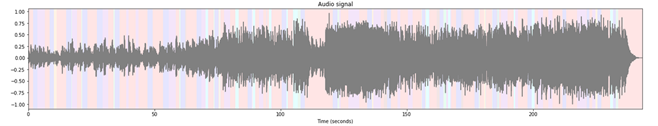
\includegraphics[scale=1]{./images/1_audio_signal.png}
 \caption{Audio Signal}
\end{figure}

\begin{figure}[H]
 \centering
 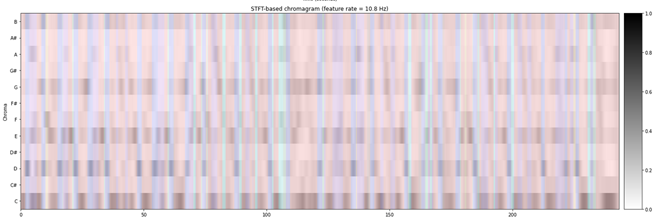
\includegraphics[scale=1]{./images/1_stft_chromagram.png}
 \caption{STFT-based Chromagram}
\end{figure}

\begin{figure}[H]
 \centering
 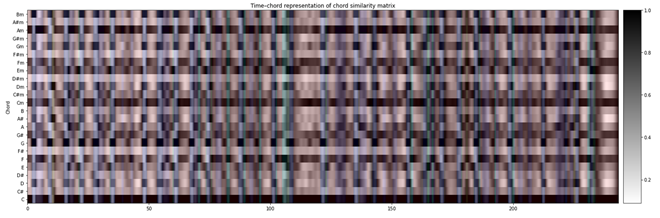
\includegraphics[scale=1]{./images/1_chord_similarity.png}
 \caption{Chord Similarity Matrix}
\end{figure}

\begin{figure}[H]
 \centering
 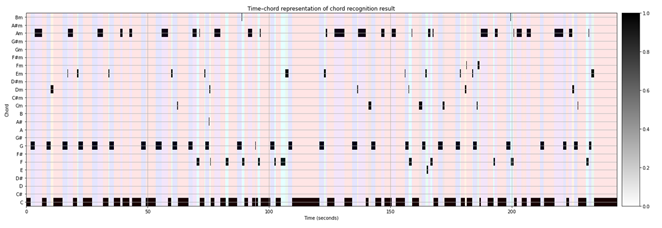
\includegraphics[scale=1]{./images/1_recognition_results.png}
 \caption{Chord Recognition Results}
\end{figure}

%----------------------------------------------------------------------------------------

\section*{\color{red}Question 2}

\begin{problem}
	\textbf{Write a function to load and preprocess a reference annotation (or ground truth) file, saved in \emph{CSV} format.}
\end{problem}

\subsection*{\color{blue}Answer}

The function should take as input the path to a CSV file and produce as output a list of ground truth chord labels, after suitable pre processing.\\
The output must be a list where each element n is the ground truth chord label for the n-th time window.

\subsection*{Ground truth processing functions}

In this paragraph is explaied each step of the preprocessing phase, focusing in particular on the reduction strategy of the chord label set.

\begin{enumerate}
	\item \verb|read_csv| - Reads the path of the .csv file.
	\item \verb|convert_segment_annotations| - The function (required in the first point, question 2) has the important role to convert the segment-based annotation into a frame-based label sequence adapted to the feature rate used for the chroma sequence.
	\item \verb|get_binary_time_chord_matrix| - The function takes as input the sequence of lables and returns the matrix with the duration (in binary rapresentation) of the various chords. It converts the labels used in the annotation file to match the chord labels used for the chord recognition
algorithm in terms of enharmonic equivalence.
\color{red} VEDI MEGLIO \color{black}
	\item \verb|normalize_chord_labels| - Important to notice is the function that normalizes chord labels. It replaces for segment-based annotation in each chord label the string ':min' by 'm' and convert flat chords into sharp chords using enharmonic equivalence. We can also see that half diminished, diminished and minor chords are classified as minor chords with the letter 'm'. Maj, sus and slash  chords are classified as major chords (' '). This is done by using Python's \textit{regex} (regular expressions). In this way we implemented the reduction strategy of the chord label set.
\end{enumerate}

\subsection*{Ground truth reading implementation}

The role of this function is to load and preprocess a reference annotation (or ground truth) file, saved in CSV format. The function \verb|read_ground_truth| should takes as input the path to a CSV file and produce as output a list of ground truth chord labels, after suitable pre processing. The output is a list where each n-th element is the ground truth chord label for the time window n. 

The function converts segment-based chord annotation into various formats and returns a frame by frame reference chords label sequence, the binary time-chord matrix representation of the reference chords label sequence,the original reference annotations given in seconds, the normalized reference annotations given in seconds.

\subsection*{Perform ground truth reading}

In this section the code performs ground truth reading, plotting the results of chord recognition.

\begin{figure}[H]
 \centering
 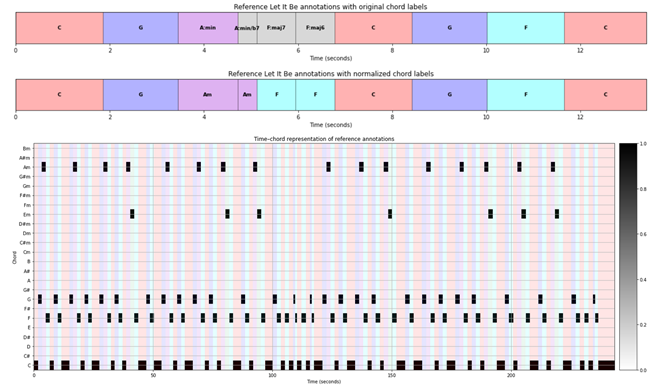
\includegraphics[scale=1]{./images/2_reference_annotations.png}
\end{figure}

%----------------------------------------------------------------------------------------

\section*{\color{red}Question 3}

\begin{problem}
	\textbf{Propose a metric for evaluating the template based chord recognition algorithm.}
\end{problem}

\subsection*{\color{blue}Answer}

In this section we define a function that takes as input the list of predicted chord labels, the list of ground truth chord labels and computes the proposed metric value: \verb|compute_eval_measures|.

A metric is a scalar number that expresses how good is the algorithm in performing the task of chord recognition.\\

We now introduce a simple evaluation measure. Recall that, given a chroma sequence \(X=(x_1,x_2,…,x_N)\) and a set \( \Lambda :=[C,C\#,…,B,Cm,Cm\#,…,Bm] \)\\

In the context of music structure analysis, we introduce evaluation measures that are used in general information retrieval. We now adapt these notions to our chord recognition scenario. First, we define the set of items to be $L=[1:N] \times \Lambda$. In particular, the non-chord label N is left unconsidered. Then:
$L_+^(Ref) := \{(n,\lambda_n^(Ref)) \in L:n\in[1:N]\}$ are the positive (or relevant items) and $L_+^(Est) :=\{(n,\lambda_n^(Est)) \in L:n\in[1:N]\}$

are the items estimated as positive (or retrieved items). With these notions, an item (n,$\lambda_n$) is called a true positive (TP) in the case that the label is correct (i.e., $\lambda_n$=$\lambda_n^(Ref)$). Otherwise, (n,$\lambda_n$) is called a false positive (FP) and (n,$\lambda_n^(Ref)$) a false negative (FN). All other items in I are called true negative. With these notions, one can define the standard precision (P), recall (R), and F-measure (F):

\[P=(\#TP)/(\#TP + \#FP)\]
\[R=(\#TP)/(\#TP + \#FN)\]
\[F=(2PR)/(P + R)\]

In the way we have formulated our chord recognition problem so far, we have exactly one label per frame in the reference as well as in the estimation. From this follows that \#FP=\#FN and that the definition of accuracy coincides with precision, recall, and F-measure. This is why in the function we use as measure the precision P. If \#TP=0, the precision is setted to the default value 0.

\subsection*{Metric evaluation implementation}

\color{red}Report \verb|compute_eval_measures| Python code\color{black}

\verb|compute_eval_measures| - The function takes as input the binary time-chord matrix representation of the reference chords label sequence and the binary chord similarity matrix containing maximizing chord.
It implements the metric (precision) defined previously by calculating the cardinality (\textit{np.sum}) of TPs (true positives), FPs (false positives), FNs (false negatives). If the numerator (\#TP) is bigger than value 0, the precision value is calculated as defined before.

This function implements exactly the precision measure as said in the previous paragraph.

\subsection*{Perform metric evaluation}

\color{red}Improve description\color{black}

We compute the evaluation for the song "Let it be" by Beatles.
Using the STFT-based chromagram in combination with the template-based chord recognizer, we obtained a precision of F=60,27\%. In fact, as the visualization shows, there are many sudden jumps between chord labels. We could optimize this result by choosing the optimal parameters setted at the beginning, but this won't be the best result.

\begin{figure}[H]
 \centering
 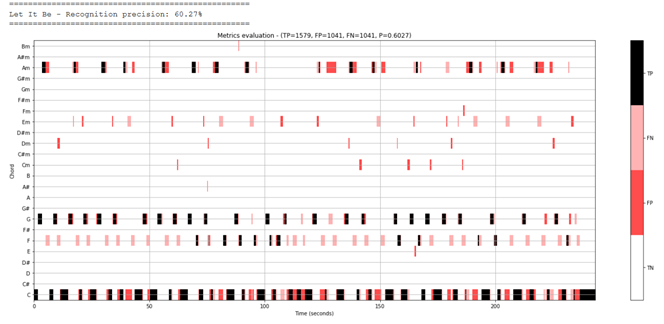
\includegraphics[scale=1]{./images/3_let_it_be_metrics.png}
 \caption{Let It Be - Metrics Evaluation}
\end{figure}

\begin{problem}
	Can you imagine a musically informed strategy that weights diferently mismatch errors of
the chord recognition algorithm?
\end{problem}

\subsection*{\color{blue}Answer}

\color{red}Manca risposta a questa domanda!\color{black}
Introduces a kind of context-aware postfiltering.

%----------------------------------------------------------------------------------------

\section*{\color{red}Question 4}

\begin{problem}
	\textbf{Compute the proposed metric for the remaining 3 songs.}
\end{problem}

\subsection*{\color{blue}Answer}
\color{red}Improve description\color{black}

We compute also the proposed metric for the remaining 3 songs.
Averaging these numbers on the song level yields a mean precision P=60.48\%. The value P=60.27\% that we found in "Let it be" is very similar to the mean; we can say that this is still due to sudden jumps between chord labels. With HMM we can obtain P=78,5\%, the value one also obtains for the entire Beatles collections (180 songs). More recent data-driven chord recognition approaches achieve recognition rates between 80 and 90 percent for the Beatles collection. In general, such numbers need to be taken with caution, since they only give limited insights into the complexity of the dataset.

\begin{figure}[H]
 \centering
 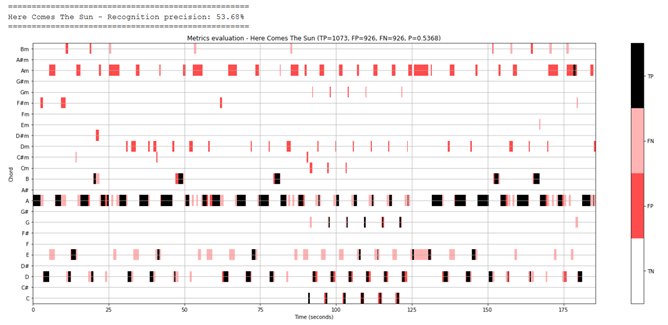
\includegraphics[scale=1]{./images/4_here_comes_the_sun_metrics.png}
 \caption{Here Comes The Sun}
\end{figure}

\begin{figure}[H]
 \centering
 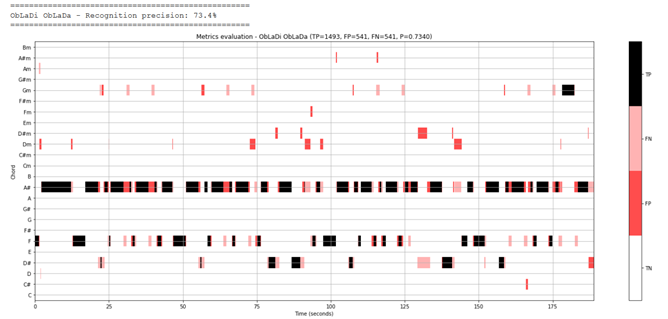
\includegraphics[scale=1]{./images/4_obladi_oblada_metrics.png}
 \caption{ObLaDì ObLada}
\end{figure}

\begin{figure}[H]
 \centering
 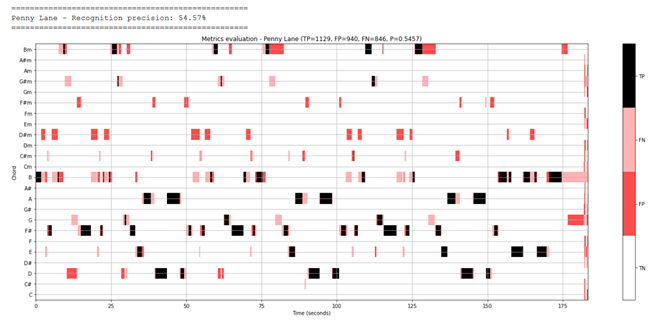
\includegraphics[scale=1]{./images/4_penny_lane_metrics.png}
 \caption{Penny Lane}
\end{figure}

%----------------------------------------------------------------------------------------

\section*{\color{red}Question 5}

\begin{problem}
	\textbf{Analyse how algorithm parameters affect the performance of the templated based chord recognition algorithm.}
\end{problem}

\subsection*{\color{blue}Answer}

\color{red}Aggiungere descrizione su come è stata fatta l'implementazione del testing (iterate over songs dictionary and overwrite globals)\color{black}

\subsection*{Smooth filter length} 

Applying temporal smoothing using a rectangular or a Hann window can be regarded as bandwise lowpass filtering, which attenuates fast temporal fluctuations in the feature representation. This allows the chord estimation to be much more precise and not be affected by high frequencies. \\
We consider the following vector of values [0,30,60]: we can see an increase in accuracy up to 30 and then a substantial settlement with a slight decrease. The graphs have similar trends.\\
We can deduce that around the value 30 the precision of our algorithm will be higher. However, it is not particularly high. To do this it will also be necessary to observe which are the best values for the other parameters that the algorithm is using. \\

\begin{figure}[H]
 \centering
 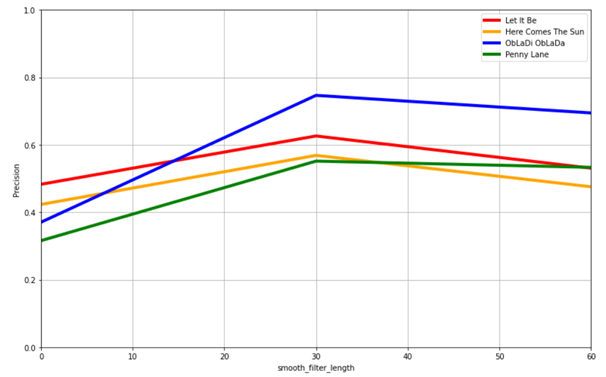
\includegraphics[scale=1]{./images/5_smooth_precision.png}
 \caption{Smooth filter length}
\end{figure}

\subsection*{Down sampling factor}

Often, after considering the smooth filter length, to increase the efficiency of subsequent processing and analysis steps, one decimates the smoothed representation by keeping only every H-th feature, where  \(H \in N\) is a suitable constant (typically much smaller than the window length L). This decimation, which is also referred to as downsampling, reduces the feature rate by a factor H.\\
We take into account these values: [0, 10, 100]: the more the downsampling factor is increased, the more you reduce the feature rate and the less you read the harmonic content (in larger steps). If chosen high, inconsistently with the window length, the precision decreases.
It's good to use it in combination with the smoothing filter for efficiency. In this case 10 or less can be a good value. 

\begin{figure}[H]
 \centering
 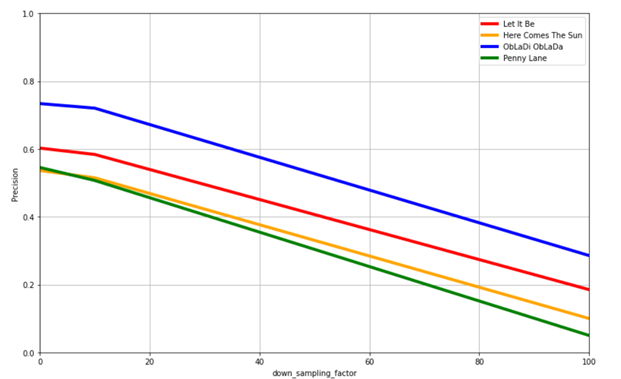
\includegraphics[scale=1]{./images/5_down_sampling_precision.png}
 \caption{Down sampling factor}
\end{figure}

\subsection*{Window length}

We consider the following vector of values of window lengths [2048, 8192, 32768]:  using an analysis window with a short duration , each chroma frame contains the onsets of at most one note. Even though the sound of each note may last much longer than the notated duration, the harmonic content of each frame is dominated by only one or two notes. This explains the misclassifications and many chord label changes in the recognition result of the first setting. \\
An obvious strategy for improving the chord recognition result is to use larger window sizes. Anyway, the larger analysis windows smooth out the originally sharp transitions between different chords, which may introduce problems at chord changes.\\

\begin{figure}[H]
 \centering
 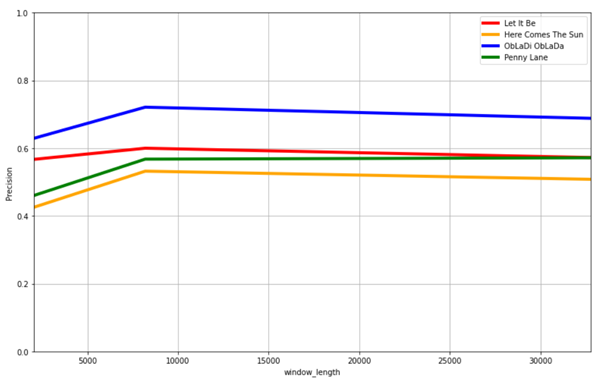
\includegraphics[scale=1]{./images/5_window_precision.png}
 \caption{Window length}
\end{figure}

%----------------------------------------------------------------------------------------

\end{document}
